\documentclass[preprint,10pt]{elsarticle}

\usepackage{amssymb}
\usepackage{amsmath}
\usepackage{lineno}

\usepackage{epstopdf}
\usepackage{epsfig}
\usepackage{setspace}
\usepackage{hyperref}

\newcommand{\be}{\begin{equation}}
\newcommand{\ee}{\end{equation}}
\newcommand{\beq}{\begin{eqnarray}}
\newcommand{\eeq}{\end{eqnarray}}
\newcommand{\ba}{\begin{eqnarray}}
\newcommand{\ea}{\end{eqnarray}}

\newcommand{\ua}{{\bf u}_\alpha}
\newcommand{\utwo}{\overline{\bf u}_2}
\setcounter{MaxMatrixCols}{24}

\journal{Coastal Engineering}

\begin{document}


%\title{Model derivations}


\begin{center}
{\bf \Huge FUNWAVE modeling of the Canada experiments}
\\
\vspace{1cm}
March 8, 2025
\end{center}

\section*{Important links}

1) \href{https://github.com/fengyanshi/Canada_Experiment}{Entire Package}

2)  \href{https://github.com/fengyanshi/Canada_Experiment/tree/main/documentation}{This documentation}

3)  \href{https://github.com/fengyanshi/Canada_Experiment/tree/main/data}{Data and preparation directory}

4)  \href{https://github.com/fengyanshi/Canada_Experiment/tree/main/data}{Data and preparation directory}

5)  \href{https://github.com/fengyanshi/Canada_Experiment/tree/main/references}{References}

\section*{Purposes}

1) provide a procedure for conducting numerical simulations of the experiments using FUNWAVE-TVD

2) preprocessing for model grids

3) model setups

4) methods of diagnosing numerical results

5) postprocessing results
  

\section*{modeling procedure}

1) generate grids. run plot\_profile\_caseX.m in /data/preprocessing/

2) compile the code in /FUNWAVE-TVD/model\_work using Makefile

3) run each case in /FUNWAVE-TVD/model\_work 
 
 For example, >mpirun -np 8 ./funwave input\_01\_01.txt 
 
 The input file is defined as input\_CaseNumber\_TrialNumber.txt
 
 4) postprocessing in  /FUNWAVE-TVD/postprocessing

For example, run Case1\_Trial01.m


\section*{diagnosing hydrodynamics and sediment transport}

See Figure 1. 

 \begin{figure}
\begin{center}
 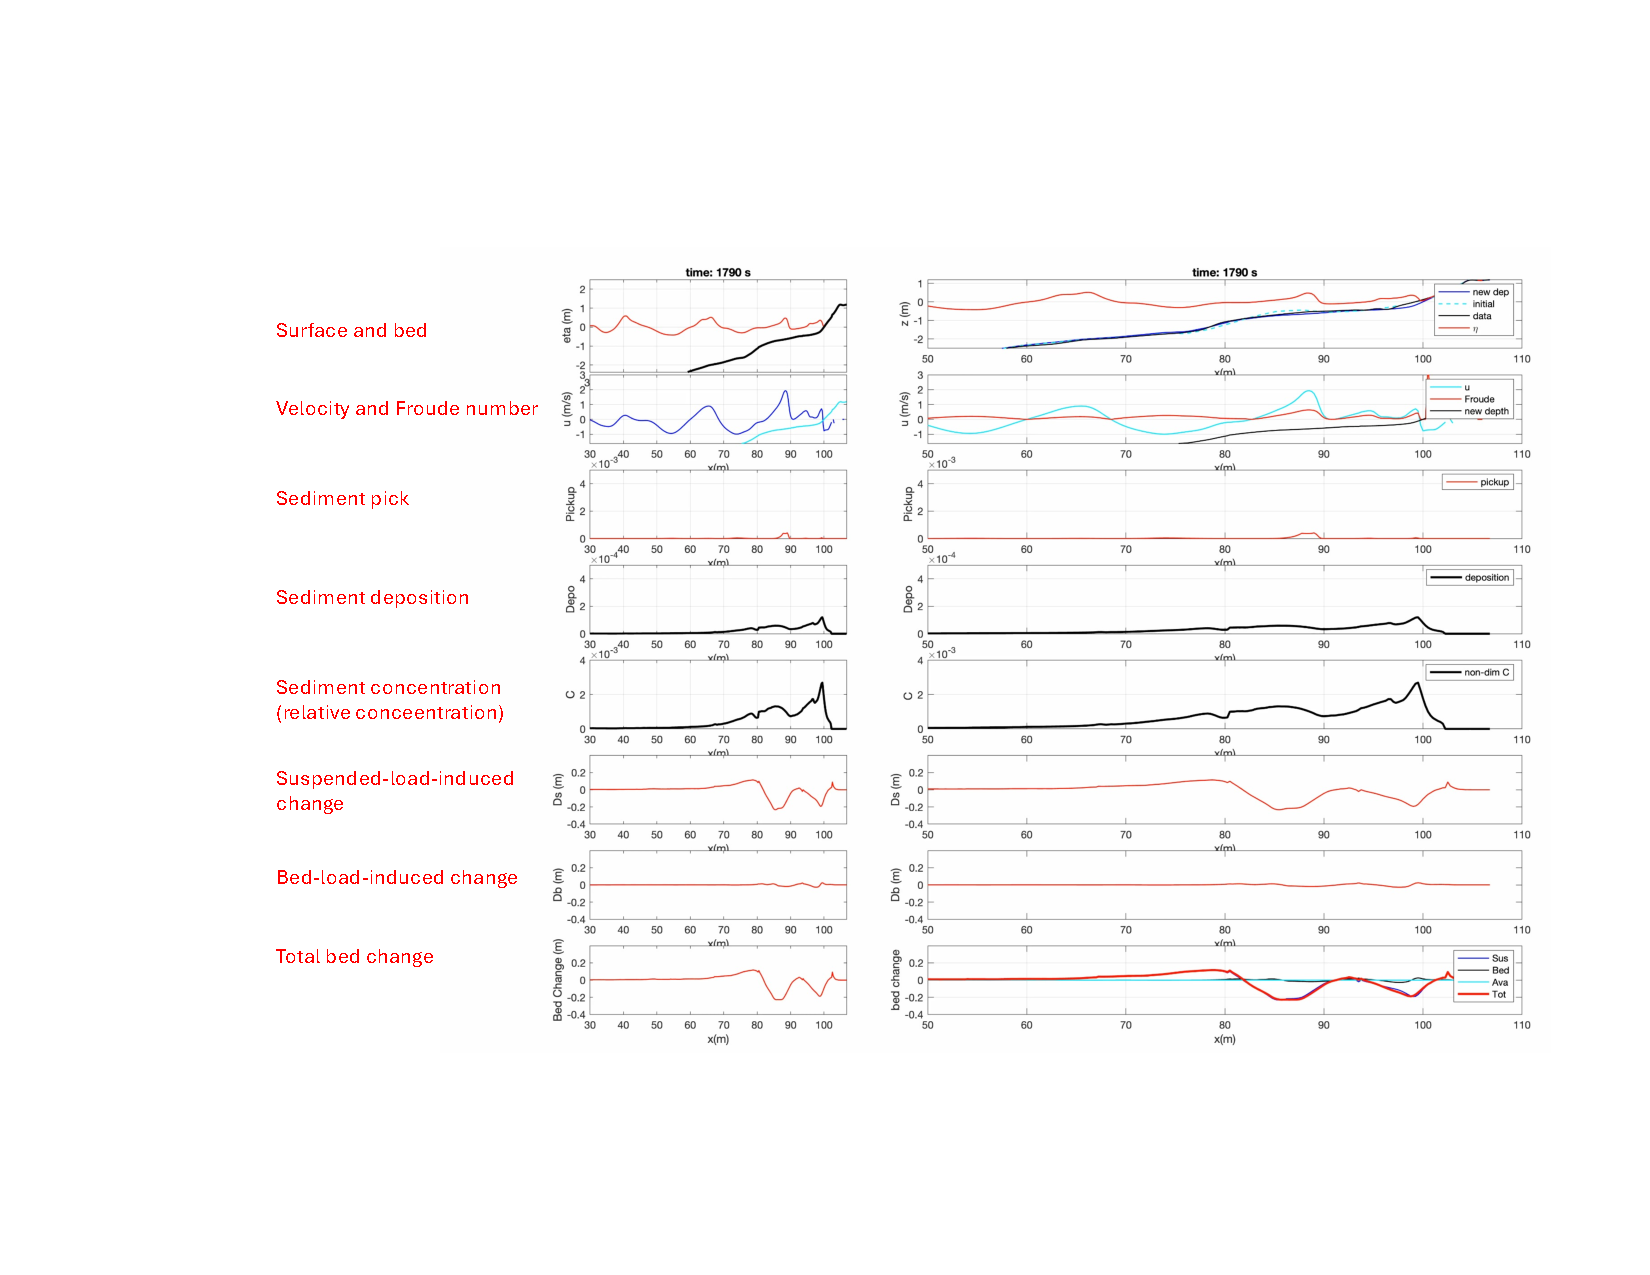
\includegraphics[width=1.0\textwidth]{diagnose.pdf}
 \caption{Example of diagnosing program. }
 \label{lineargrid}
 \end{center}
 \end{figure}

\section*{Initial assessment}  

The model/data comparisons of morphological change are generally unsatisfactory. There are several potential causes for the poor comparisons

1) the model was not tuned 

2) some profile changes don't look consistent with hydrodynamic conditions. Possibly the model loaded or compared wrong data. In some cases, mass is not conserved in the lab data. 

3) the model is inappropriate for modeling CASE 6 in which waves are too long (T=12s) for wave generation in about 2m depth.  

4) the model is efficient. Each case costs 30s -- 60s on my MAC with 8 cores. 

\section*{Suggestions}  

1) check the profile data first. I used the smoothed profiles made by Sahar

2) the model needs to be tuned in a typical case, and the same parameters can be applied to all other cases. Suggest using an automated program in linux/unix system. I think Windows system can also have the option. 

3) use the diagnosing script when tuning the model

4) model/data comparison of waves should be conducted at surfzone locations.  


\newpage

 \begin{figure}
\begin{center}
 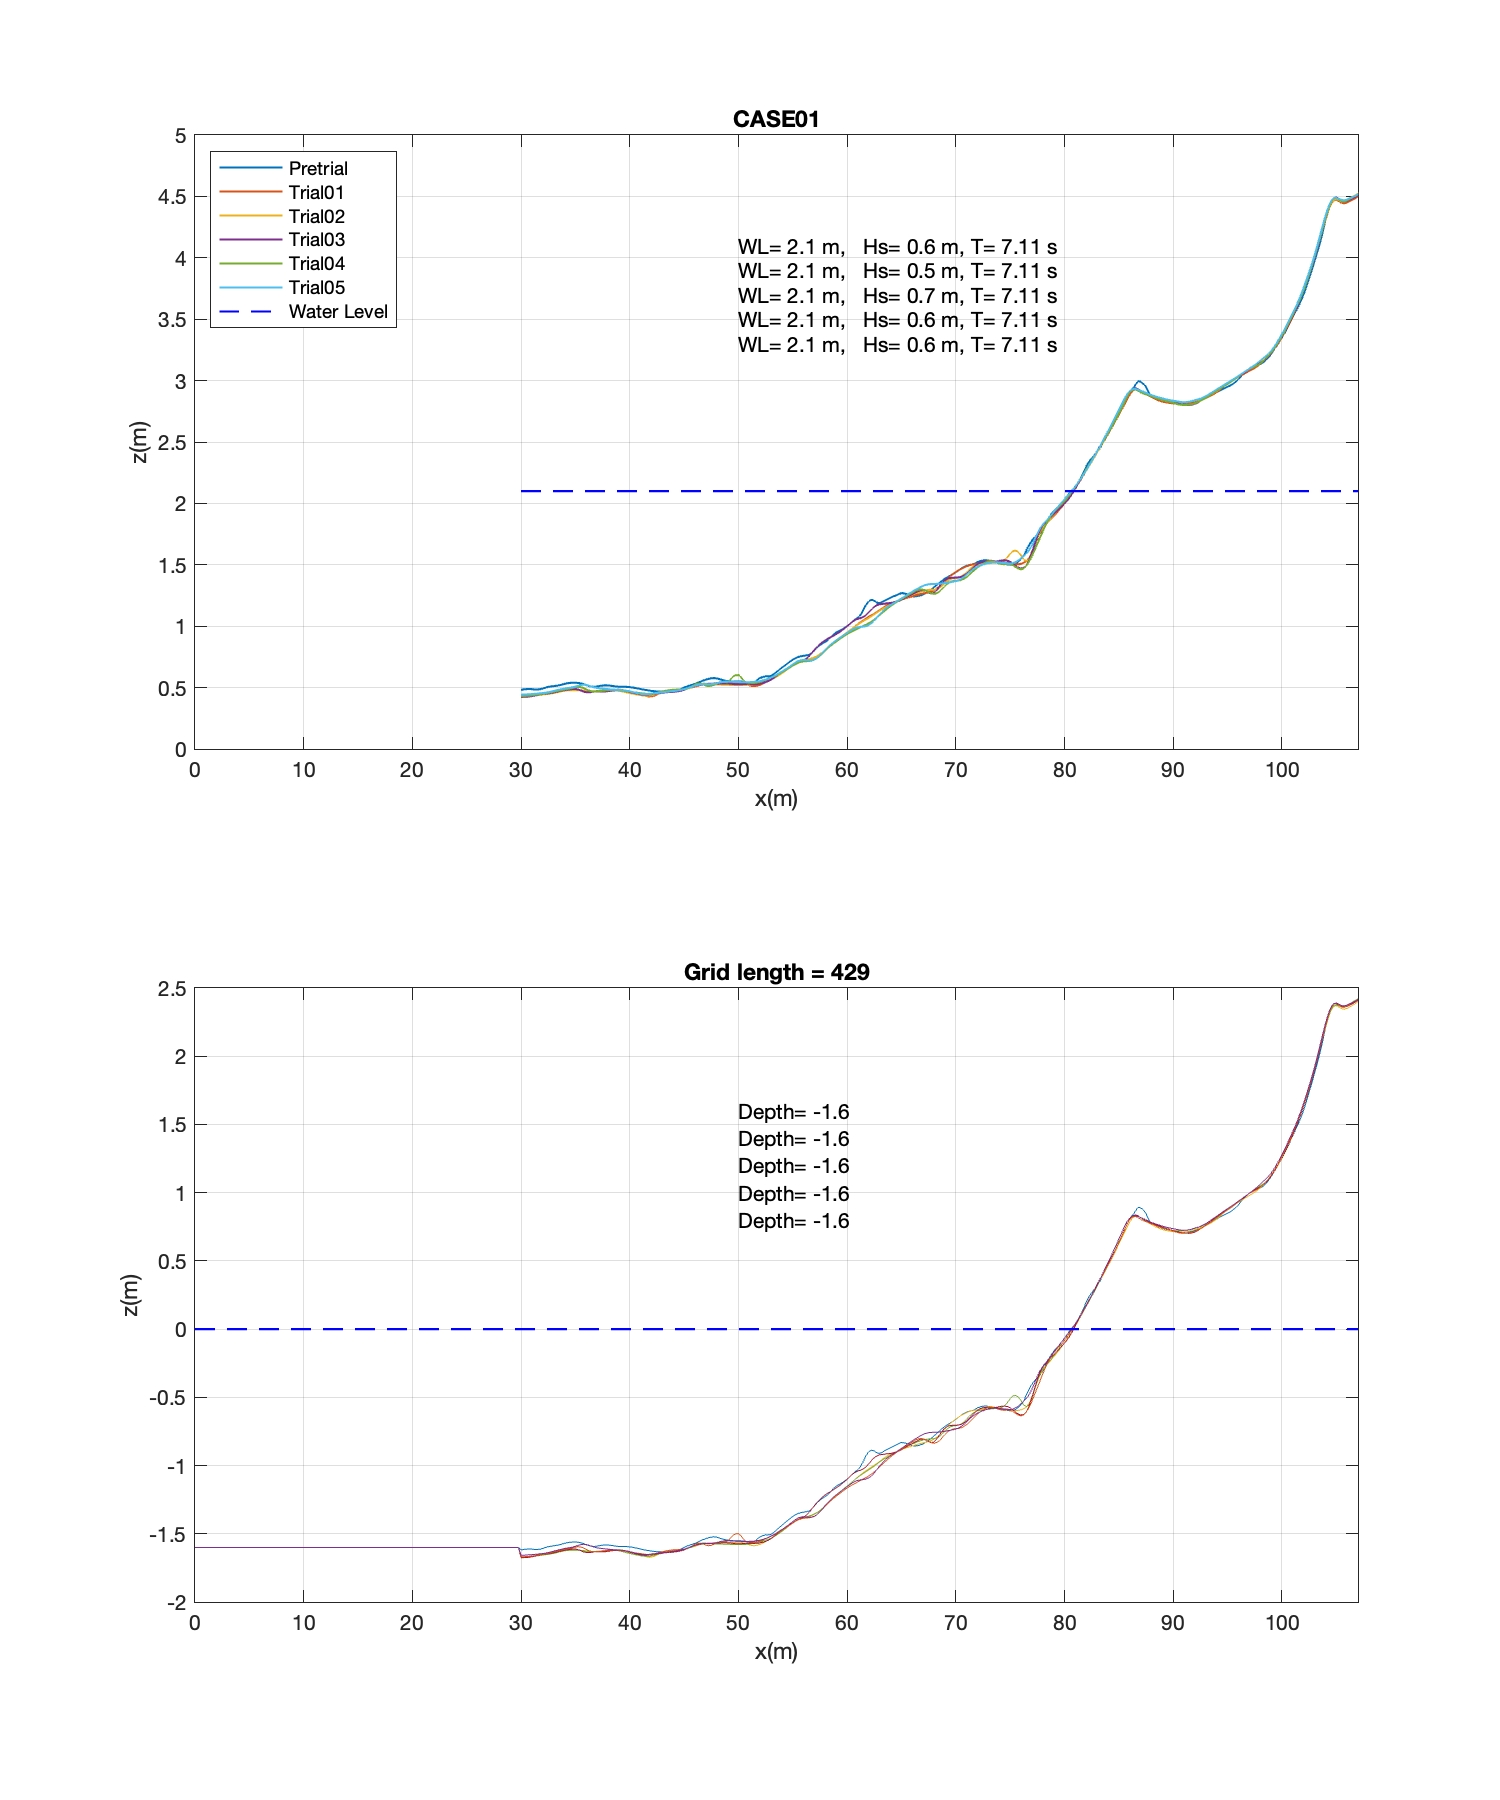
\includegraphics[width=0.8\textwidth]{../data/preprocessing/plots/CASE01.jpg}
 \caption{CASE01, data (top panel), model grid (bottom panel).}
 \label{lineargrid}
 \end{center}
 \end{figure}
 
 \begin{figure}
\begin{center}
 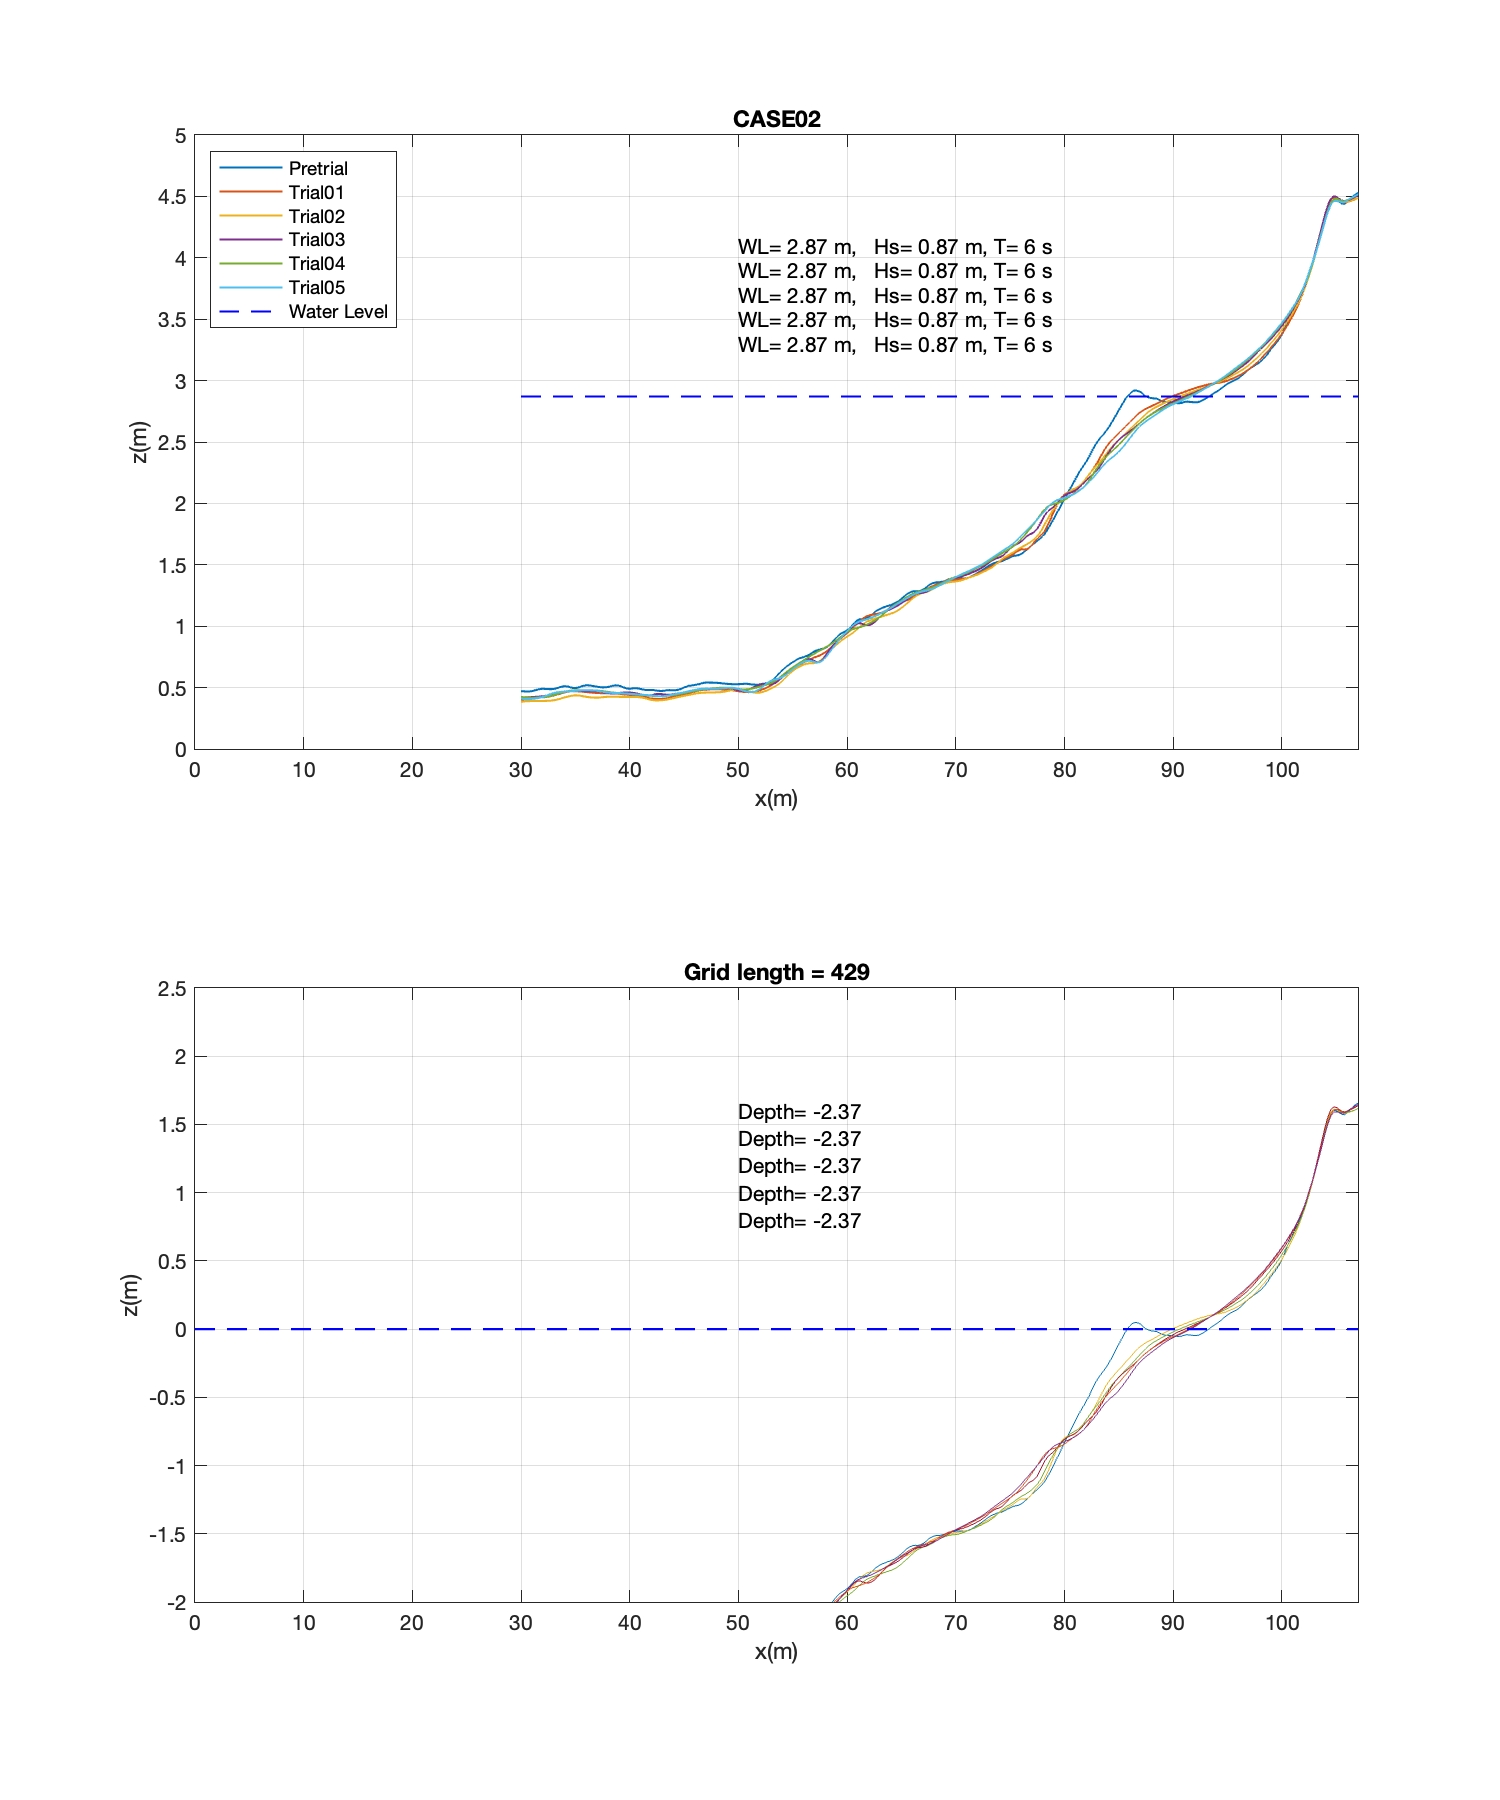
\includegraphics[width=1.0\textwidth]{../data/preprocessing/plots/CASE02.jpg}
 \caption{CASE02, data (top panel), model grid (bottom panel).}
 \label{lineargrid}
 \end{center}
 \end{figure}

 \begin{figure}
\begin{center}
 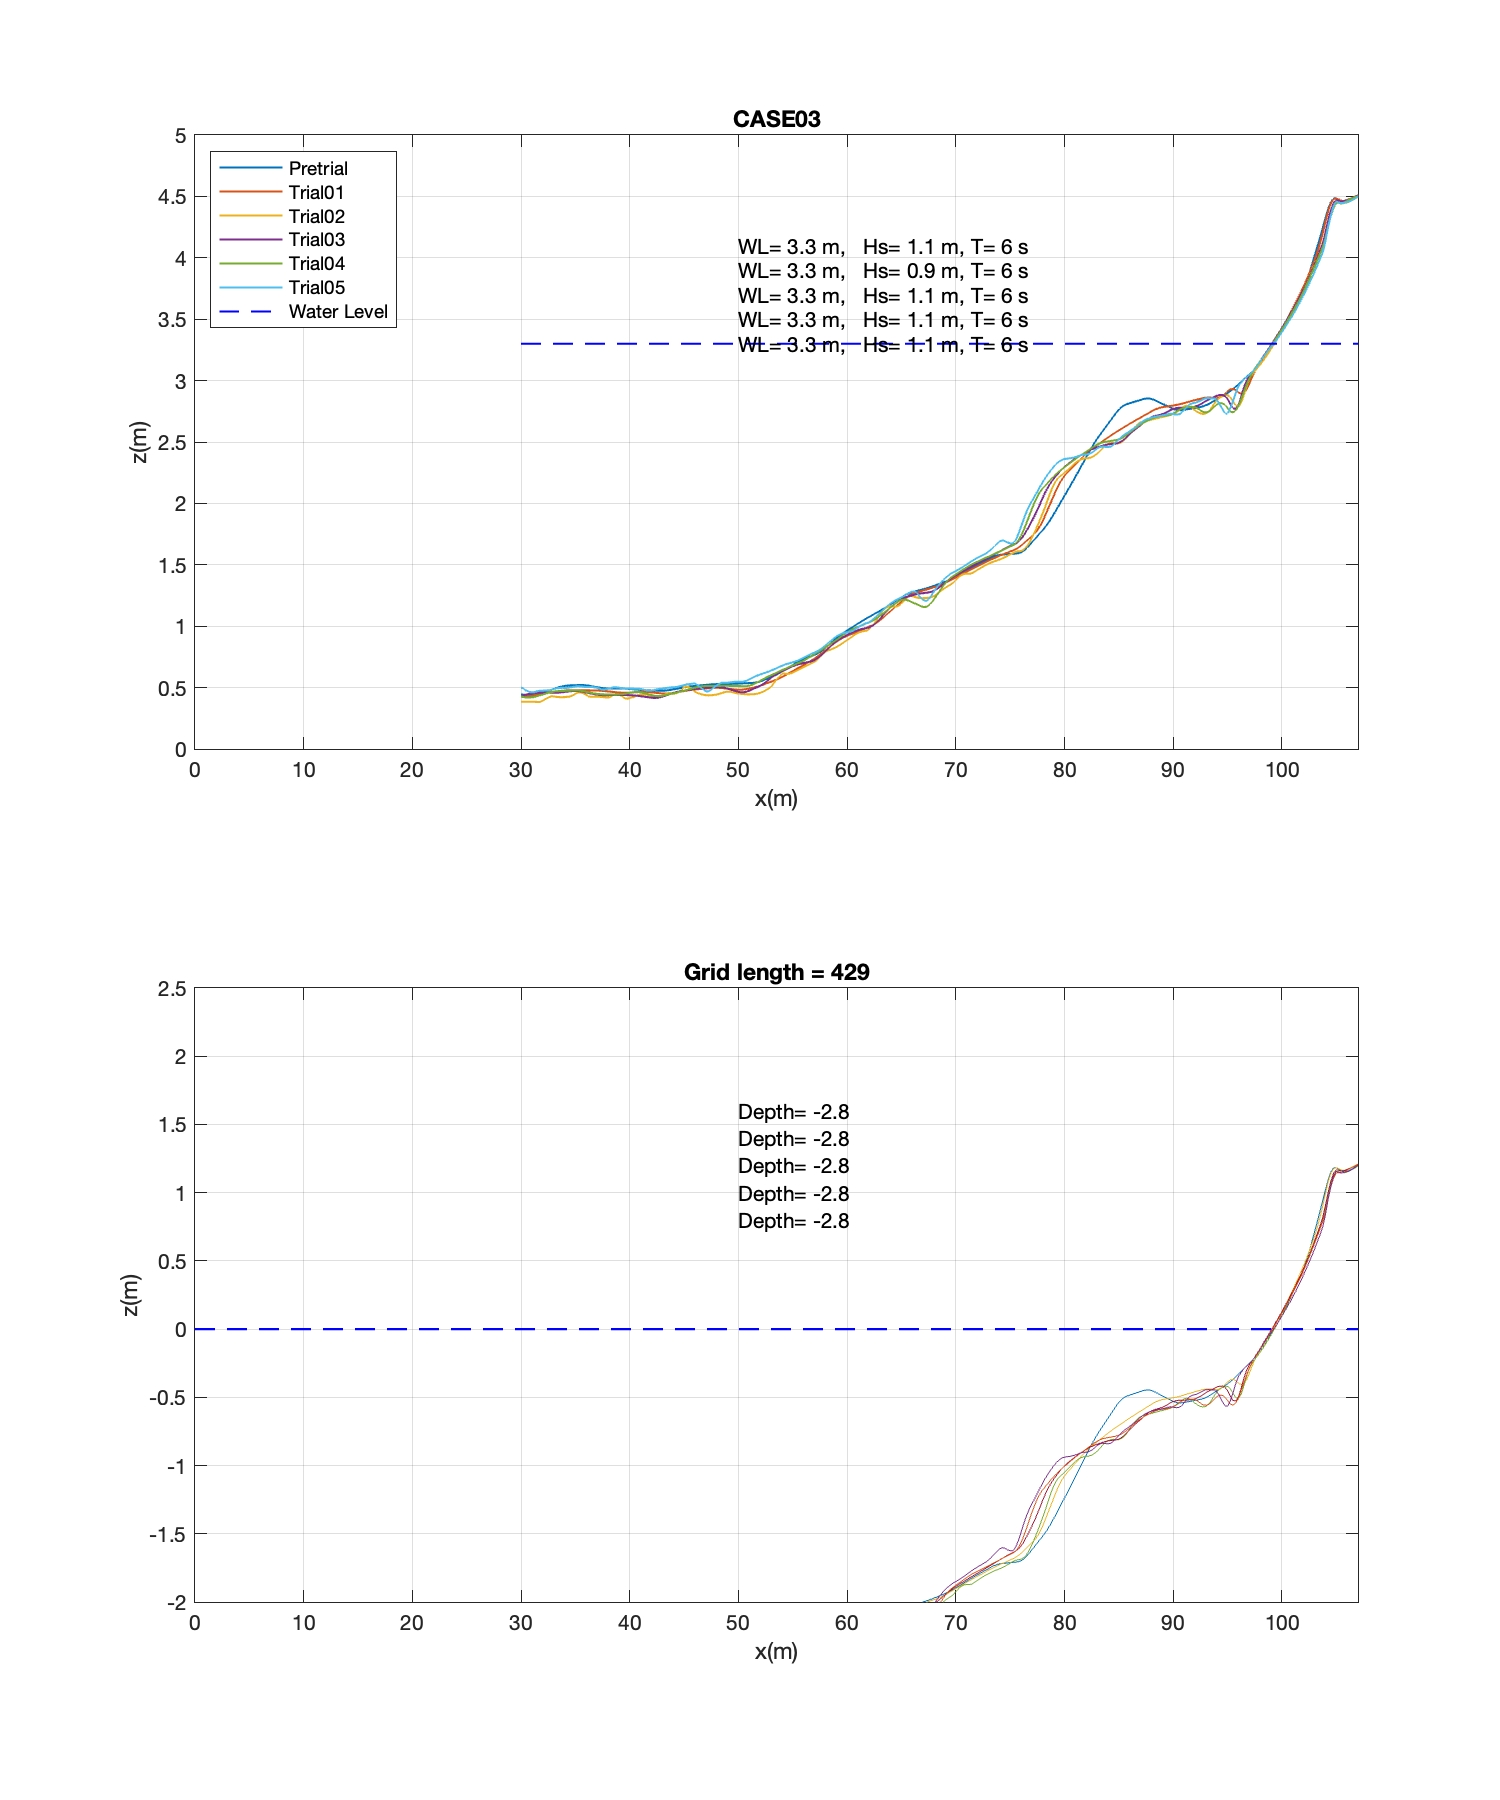
\includegraphics[width=1.0\textwidth]{../data/preprocessing/plots/CASE03.jpg}
 \caption{CASE03, data (top panel), model grid (bottom panel).}
 \label{lineargrid}
 \end{center}
 \end{figure}

 \begin{figure}
\begin{center}
 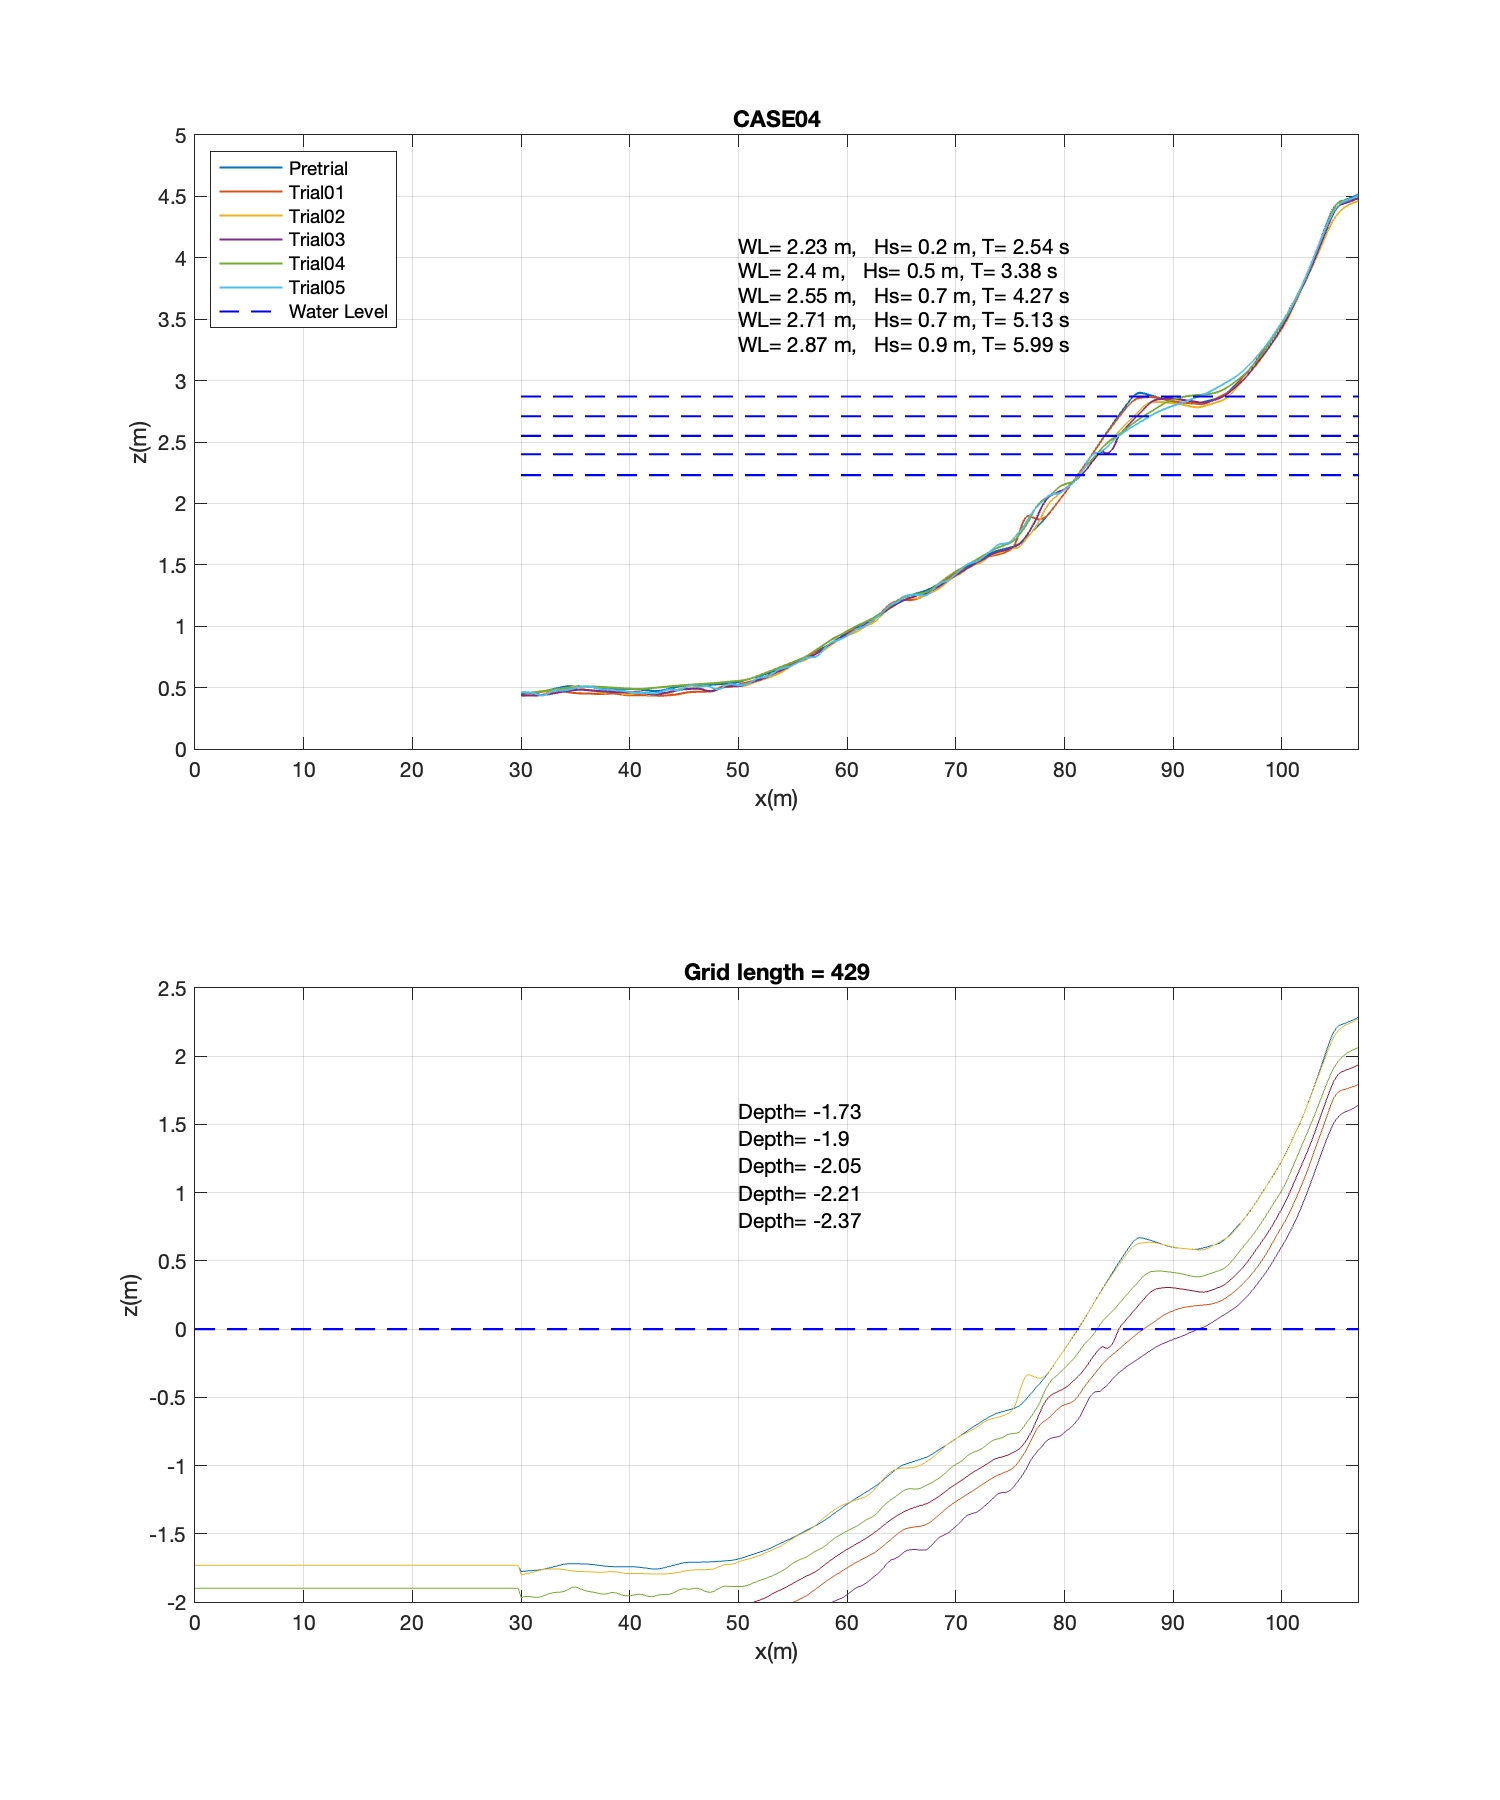
\includegraphics[width=1.0\textwidth]{../data/preprocessing/plots/CASE04.jpg}
 \caption{CASE04, data (top panel), model grid (bottom panel).}
 \label{lineargrid}
 \end{center}
 \end{figure}

 \begin{figure}
\begin{center}
 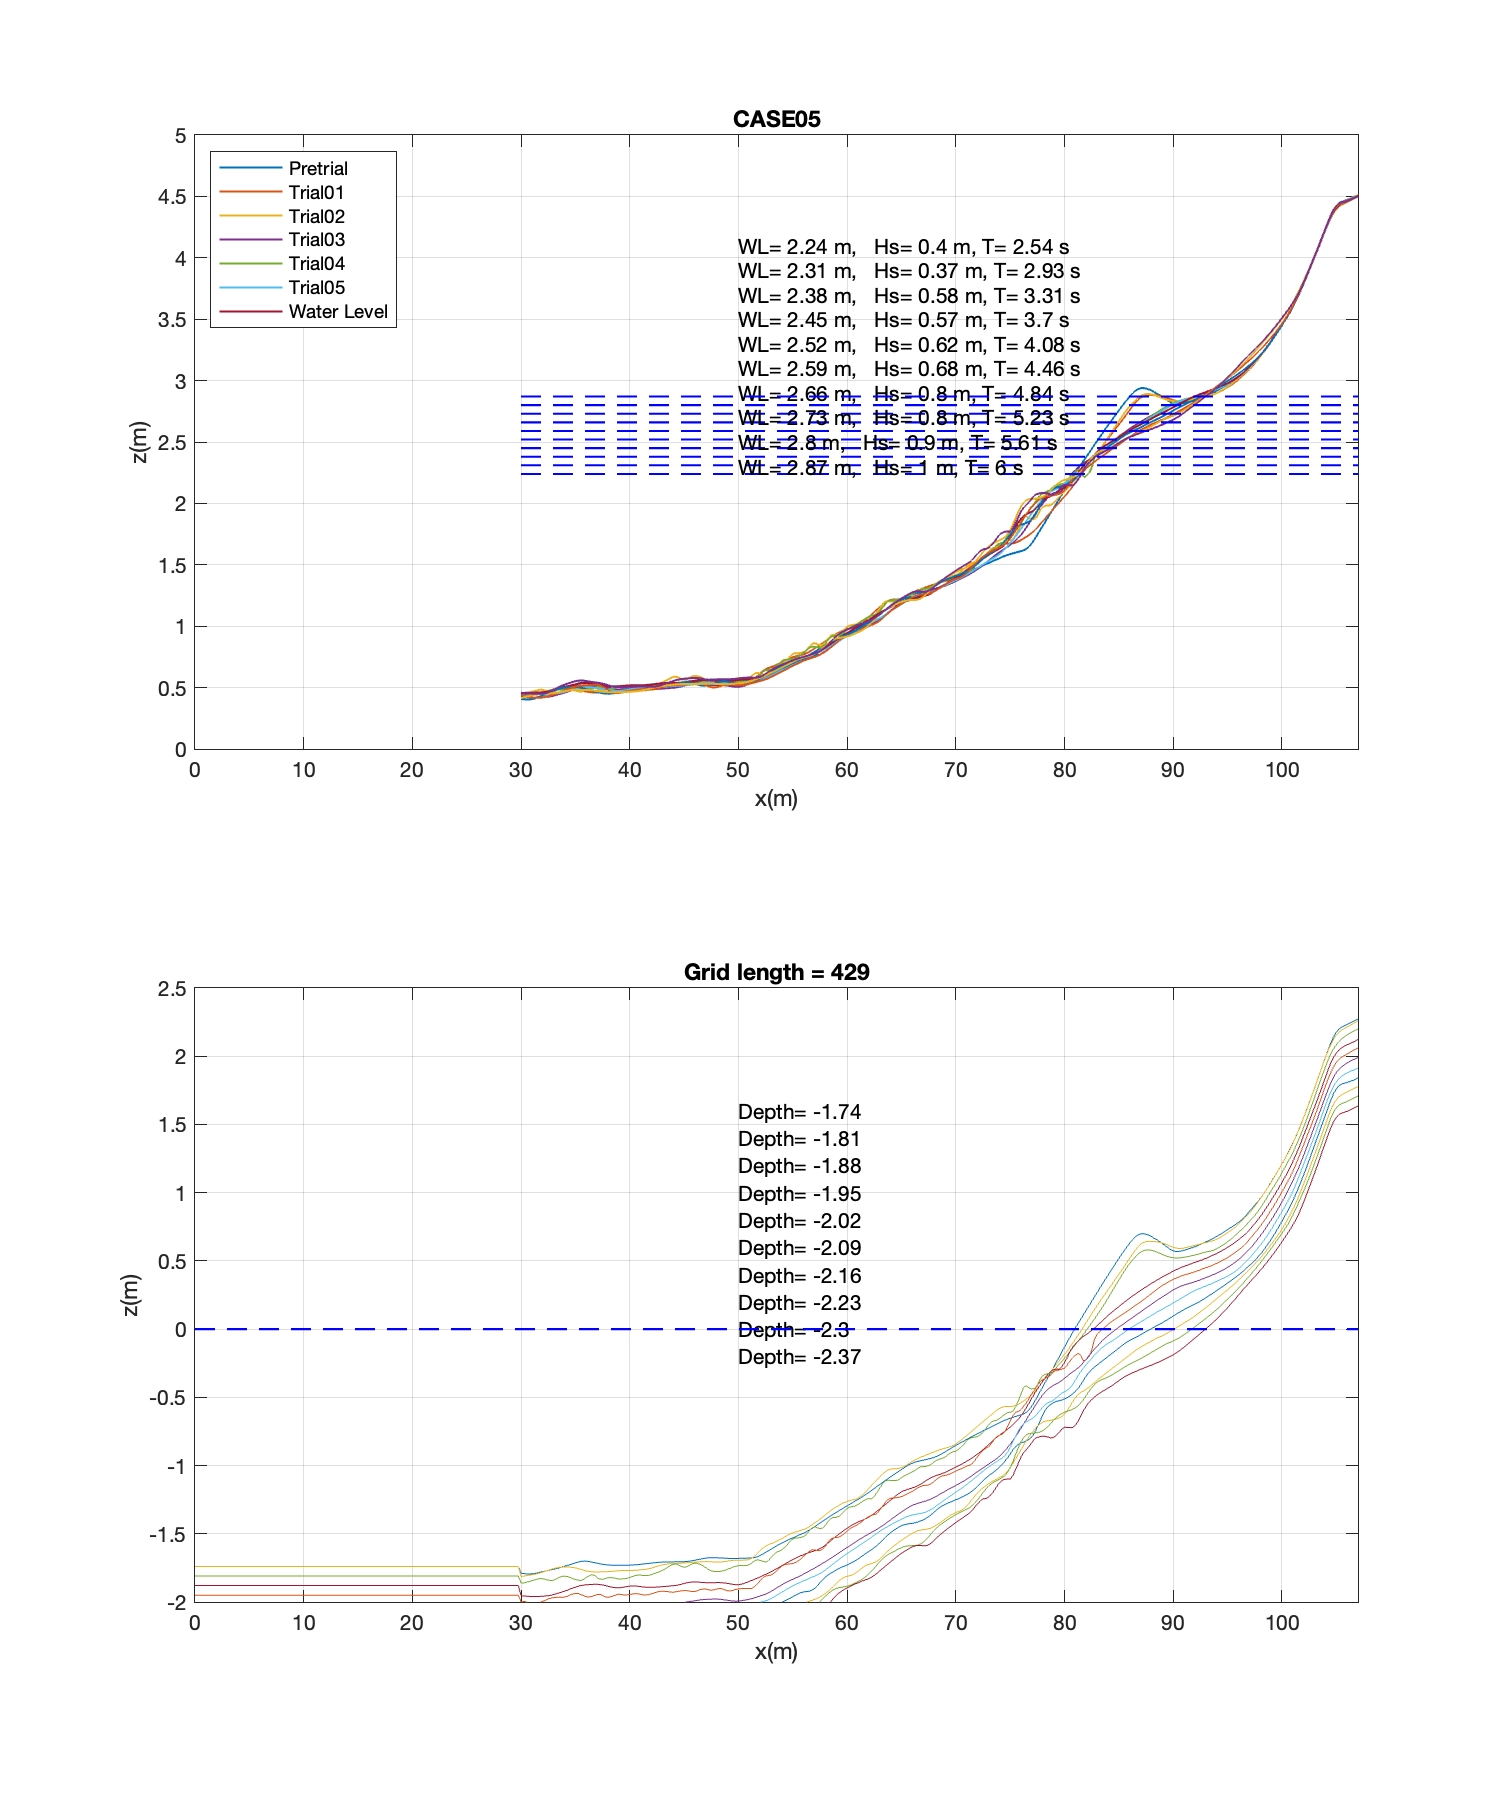
\includegraphics[width=1.0\textwidth]{../data/preprocessing/plots/CASE05.jpg}
 \caption{CASE05, data (top panel), model grid (bottom panel).}
 \label{lineargrid}
 \end{center}
 \end{figure}

 \begin{figure}
\begin{center}
 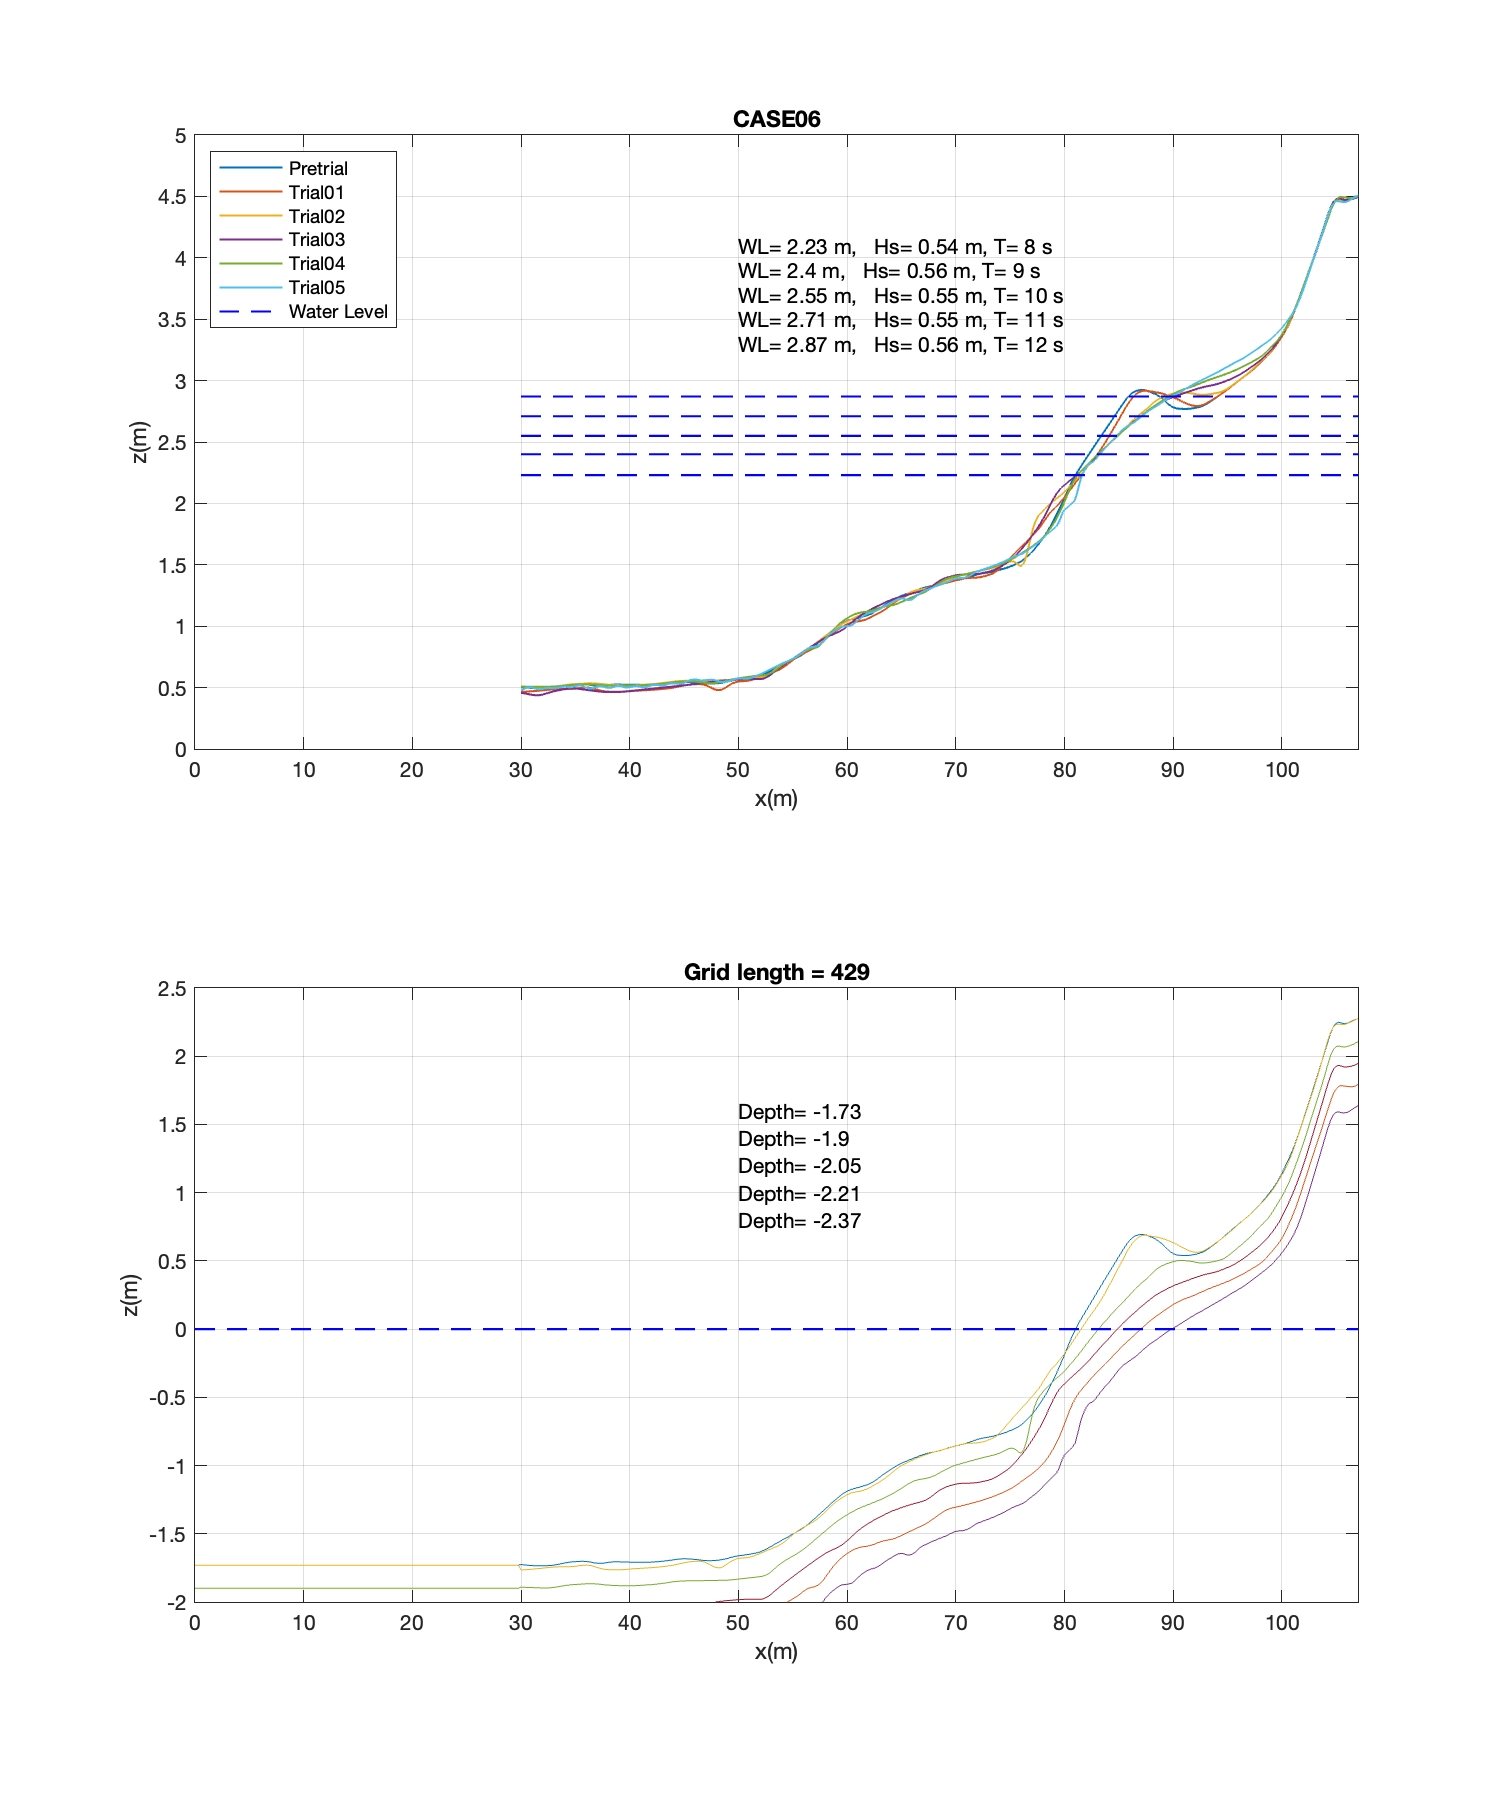
\includegraphics[width=1.0\textwidth]{../data/preprocessing/plots/CASE06.jpg}
 \caption{CASE06, data (top panel), model grid (bottom panel).}
 \label{lineargrid}
 \end{center}
 \end{figure}

 \newpage
  
 \begin{figure}
\begin{center}
 \includegraphics[width=0.8\textwidth]{../FUNWAVE-TVD/postprocessing/plots/CASE01_Trial01.jpg}
 \caption{CASE01, Trial01}
 \label{lineargrid}
 \end{center}
 \end{figure}

\begin{figure}
\begin{center}
 \includegraphics[width=0.8\textwidth]{../FUNWAVE-TVD/postprocessing/plots/CASE01_Trial02.jpg}
 \caption{CASE01, Trial02}
 \label{lineargrid}
 \end{center}
 \end{figure}

\begin{figure}
\begin{center}
 \includegraphics[width=0.8\textwidth]{../FUNWAVE-TVD/postprocessing/plots/CASE01_Trial03.jpg}
 \caption{CASE01, Trial03}
 \label{lineargrid}
 \end{center}
 \end{figure}
 
\begin{figure}
\begin{center}
 \includegraphics[width=0.8\textwidth]{../FUNWAVE-TVD/postprocessing/plots/CASE01_Trial04.jpg}
 \caption{CASE01, Trial04}
 \label{lineargrid}
 \end{center}
 \end{figure}

\begin{figure}
\begin{center}
 \includegraphics[width=0.8\textwidth]{../FUNWAVE-TVD/postprocessing/plots/CASE01_Trial05.jpg}
 \caption{CASE01, Trial05}
 \label{lineargrid}
 \end{center}
 \end{figure}

\newpage

 \begin{figure}
\begin{center}
 \includegraphics[width=0.8\textwidth]{../FUNWAVE-TVD/postprocessing/plots/CASE02_Trial01.jpg}
 \caption{CASE02, Trial01}
 \label{lineargrid}
 \end{center}
 \end{figure}

\begin{figure}
\begin{center}
 \includegraphics[width=0.8\textwidth]{../FUNWAVE-TVD/postprocessing/plots/CASE02_Trial02.jpg}
 \caption{CASE02, Trial02}
 \label{lineargrid}
 \end{center}
 \end{figure}

\begin{figure}
\begin{center}
 \includegraphics[width=0.8\textwidth]{../FUNWAVE-TVD/postprocessing/plots/CASE02_Trial03.jpg}
 \caption{CASE02, Trial03}
 \label{lineargrid}
 \end{center}
 \end{figure}
 
\begin{figure}
\begin{center}
 \includegraphics[width=0.8\textwidth]{../FUNWAVE-TVD/postprocessing/plots/CASE02_Trial04.jpg}
 \caption{CASE02, Trial04}
 \label{lineargrid}
 \end{center}
 \end{figure}

\begin{figure}
\begin{center}
 \includegraphics[width=0.8\textwidth]{../FUNWAVE-TVD/postprocessing/plots/CASE02_Trial05.jpg}
 \caption{CASE02, Trial05}
 \label{lineargrid}
 \end{center}
 \end{figure}

 \begin{figure}
\begin{center}
 \includegraphics[width=0.8\textwidth]{../FUNWAVE-TVD/postprocessing/plots/CASE03_Trial01.jpg}
 \caption{CASE03, Trial01}
 \label{lineargrid}
 \end{center}
 \end{figure}

\begin{figure}
\begin{center}
 \includegraphics[width=0.8\textwidth]{../FUNWAVE-TVD/postprocessing/plots/CASE03_Trial02.jpg}
 \caption{CASE03, Trial02}
 \label{lineargrid}
 \end{center}
 \end{figure}

\begin{figure}
\begin{center}
 \includegraphics[width=0.8\textwidth]{../FUNWAVE-TVD/postprocessing/plots/CASE03_Trial03.jpg}
 \caption{CASE03, Trial03}
 \label{lineargrid}
 \end{center}
 \end{figure}
 
\begin{figure}
\begin{center}
 \includegraphics[width=0.8\textwidth]{../FUNWAVE-TVD/postprocessing/plots/CASE03_Trial04.jpg}
 \caption{CASE03, Trial04}
 \label{lineargrid}
 \end{center}
 \end{figure}

\begin{figure}
\begin{center}
 \includegraphics[width=0.8\textwidth]{../FUNWAVE-TVD/postprocessing/plots/CASE03_Trial05.jpg}
 \caption{CASE03, Trial05}
 \label{lineargrid}
 \end{center}
 \end{figure}

 \begin{figure}
\begin{center}
 \includegraphics[width=0.8\textwidth]{../FUNWAVE-TVD/postprocessing/plots/CASE04_Trial01.jpg}
 \caption{CASE04, Trial01}
 \label{lineargrid}
 \end{center}
 \end{figure}

\begin{figure}
\begin{center}
 \includegraphics[width=0.8\textwidth]{../FUNWAVE-TVD/postprocessing/plots/CASE04_Trial02.jpg}
 \caption{CASE04, Trial02}
 \label{lineargrid}
 \end{center}
 \end{figure}

\begin{figure}
\begin{center}
 \includegraphics[width=0.8\textwidth]{../FUNWAVE-TVD/postprocessing/plots/CASE04_Trial03.jpg}
 \caption{CASE04, Trial03}
 \label{lineargrid}
 \end{center}
 \end{figure}
 
\begin{figure}
\begin{center}
 \includegraphics[width=0.8\textwidth]{../FUNWAVE-TVD/postprocessing/plots/CASE04_Trial04.jpg}
 \caption{CASE04, Trial04}
 \label{lineargrid}
 \end{center}
 \end{figure}

\begin{figure}
\begin{center}
 \includegraphics[width=0.8\textwidth]{../FUNWAVE-TVD/postprocessing/plots/CASE04_Trial05.jpg}
 \caption{CASE04, Trial05}
 \label{lineargrid}
 \end{center}
 \end{figure}

 \begin{figure}
\begin{center}
 \includegraphics[width=0.8\textwidth]{../FUNWAVE-TVD/postprocessing/plots/CASE05_Trial01.jpg}
 \caption{CASE05, Trial01}
 \label{lineargrid}
 \end{center}
 \end{figure}

\begin{figure}
\begin{center}
 \includegraphics[width=0.8\textwidth]{../FUNWAVE-TVD/postprocessing/plots/CASE05_Trial02.jpg}
 \caption{CASE05, Trial02}
 \label{lineargrid}
 \end{center}
 \end{figure}

\begin{figure}
\begin{center}
 \includegraphics[width=0.8\textwidth]{../FUNWAVE-TVD/postprocessing/plots/CASE05_Trial03.jpg}
 \caption{CASE05, Trial03}
 \label{lineargrid}
 \end{center}
 \end{figure}
 
\begin{figure}
\begin{center}
 \includegraphics[width=0.8\textwidth]{../FUNWAVE-TVD/postprocessing/plots/CASE05_Trial04.jpg}
 \caption{CASE05, Trial04}
 \label{lineargrid}
 \end{center}
 \end{figure}

\begin{figure}
\begin{center}
 \includegraphics[width=0.8\textwidth]{../FUNWAVE-TVD/postprocessing/plots/CASE05_Trial05.jpg}
 \caption{CASE05, Trial05}
 \label{lineargrid}
 \end{center}
 \end{figure}

 \begin{figure}
\begin{center}
 \includegraphics[width=0.8\textwidth]{../FUNWAVE-TVD/postprocessing/plots/CASE05_Trial06.jpg}
 \caption{CASE05, Trial06}
 \label{lineargrid}
 \end{center}
 \end{figure}

\begin{figure}
\begin{center}
 \includegraphics[width=0.8\textwidth]{../FUNWAVE-TVD/postprocessing/plots/CASE05_Trial07.jpg}
 \caption{CASE05, Trial07}
 \label{lineargrid}
 \end{center}
 \end{figure}

\begin{figure}
\begin{center}
 \includegraphics[width=0.8\textwidth]{../FUNWAVE-TVD/postprocessing/plots/CASE05_Trial08.jpg}
 \caption{CASE05, Trial08}
 \label{lineargrid}
 \end{center}
 \end{figure}
 
\begin{figure}
\begin{center}
 \includegraphics[width=0.8\textwidth]{../FUNWAVE-TVD/postprocessing/plots/CASE05_Trial09.jpg}
 \caption{CASE05, Trial09}
 \label{lineargrid}
 \end{center}
 \end{figure}

\begin{figure}
\begin{center}
 \includegraphics[width=0.8\textwidth]{../FUNWAVE-TVD/postprocessing/plots/CASE05_Trial10.jpg}
 \caption{CASE05, Trial10}
 \label{lineargrid}
 \end{center}
 \end{figure}

 \begin{figure}
\begin{center}
 \includegraphics[width=0.8\textwidth]{../FUNWAVE-TVD/postprocessing/plots/CASE06_Trial01.jpg}
 \caption{CASE06, Trial01}
 \label{lineargrid}
 \end{center}
 \end{figure}

\begin{figure}
\begin{center}
 \includegraphics[width=0.8\textwidth]{../FUNWAVE-TVD/postprocessing/plots/CASE06_Trial02.jpg}
 \caption{CASE06, Trial02}
 \label{lineargrid}
 \end{center}
 \end{figure}

\begin{figure}
\begin{center}
 \includegraphics[width=0.8\textwidth]{../FUNWAVE-TVD/postprocessing/plots/CASE06_Trial03.jpg}
 \caption{CASE06, Trial03}
 \label{lineargrid}
 \end{center}
 \end{figure}
 
\begin{figure}
\begin{center}
 \includegraphics[width=0.8\textwidth]{../FUNWAVE-TVD/postprocessing/plots/CASE06_Trial04.jpg}
 \caption{CASE06, Trial04}
 \label{lineargrid}
 \end{center}
 \end{figure}

\begin{figure}
\begin{center}
 \includegraphics[width=0.8\textwidth]{../FUNWAVE-TVD/postprocessing/plots/CASE06_Trial05.jpg}
 \caption{CASE06, Trial05}
 \label{lineargrid}
 \end{center}
 \end{figure}


\end{document}







